\documentclass[a4paper,12pt]{exam}

\makeatletter
\expandafter\providecommand\expandafter*\csname ver@framed.sty\endcsname
{2003/07/21 v0.8a Simulated by exam}
\makeatother

\usepackage{xcolor}
\usepackage{minted}
\usepackage[utf8]{inputenc}
\usepackage{tikz}
\usepackage{caption}
\usepackage{gensymb}
\usepackage{lmodern}
\usepackage{multirow}
\usepackage{booktabs}
\usepackage{array}
\usepackage{adjustbox}
\usepackage{upquote}
\usepackage{amsmath}
\usepackage[hidelinks]{hyperref}
\usetikzlibrary{mindmap,shadows, shapes, arrows, positioning}

\AtBeginEnvironment{minted}{\renewcommand{\fcolorbox}[4][]{#4}}

\renewcommand{\refname}{\selectfont\normalsize References} 
\pagestyle{headandfoot}

\header{\textbf{Problem Sheet: Graph Databases}}{}{Graph Theory}
\footer{}{Page \thepage\ of \numpages}{}
\marksnotpoints
\pointsinrightmargin

\begin{coverpages}
\end{coverpages}

\begin{document}

\printanswers

\noindent
The following questions are related to the graph database system Neo4j~\cite{neo4j}, and the included Movie database~\cite{moviedb}.

\begin{questions}

\question
Create three nodes in Cypher to represent three friends -- Jack, Jerry and John.
\begin{solution}
  \begin{minted}{cypher}
CREATE
  (jack:User:Male {Name: "Jack"}), 
  (jerry:User:Male {Name: "Jerry"}),
  (john:User:Male {Name: "John"})

RETURN
  jack, jerry, john;
  \end{minted}
\end{solution}
  
\question
Create relationships showing that:

\begin{itemize}
  \item Jack follows Jerry on Twitter.
  \item Jack follows John on Twitter.
  \item John follows Jerry on Twitter.
\end{itemize}

\begin{solution}
  \begin{minted}{cypher}
MATCH
  (n:User {Name: "Jack"}), (m:User {Name: "Jerry"})
CREATE
  (n)-[r:FOLLOWS_TWITTER]->(m)
RETURN r;
// OR create two/three at a time:
MATCH 
  (n:User {Name: "Jack"}),
  (m:User {Name: "Jerry"}),
  (p:User {Name: "John"})
CREATE
  (n)-[r:FOLLOWS_TWITTER]->(p),
  (p)-[s:FOLLOWS_TWITTER]->(m)
RETURN
  r, s;
  \end{minted}
\end{solution}

\question
Add some information about Jack, Jerry and John:
\begin{itemize}
  \item Jack joined Twitter in May 2010.
  \item Jerry joined Twitter in June 2012.
  \item John joined Twitter in January 2016.
\end{itemize}

\begin{solution}
\begin{minted}{cypher}
MATCH (a:User {Name: "Jack"})
SET a.joinTwitter = "May 2010"
RETURN a;

MATCH
  (a:User {Name: "Jerry"})
  , (b:User {Name: "John"})
SET
  a.joinTwitter = "June 2012"
  , b.joinTwitter = "January 2016"
RETURN
  a, b;
  \end{minted}
\end{solution}

\question
Add some information about the following relationships:
\begin{itemize}
  \item Jack started following Jerry in July 2012.
  \item Jack started following John in February 2016.
  \item John started following Jerry on January 2016.
\end{itemize}

\begin{solution}
  \begin{minted}{cypher}
MATCH
  (a:User {Name: "Jack"})
  -[r:FOLLOWS_TWITTER]->
  (b:User {Name: "Jerry"})
SET
  r.started = "June 2012";
	
MATCH
  (a:User {Name: "Jack"})
  -[r:FOLLOWS_TWITTER]->
  (b:User {Name: "John"})
SET
  r.started = "February 2016";
	
MATCH
  (a:User {Name: "John"})
  -[r:FOLLOWS_TWITTER]->
  (b:User {Name: "Jerry"})
SET
  r.started = "January 2016";
  \end{minted}
\end{solution}

\question
  Create the following graph in Cypher:
  \begin{center}
  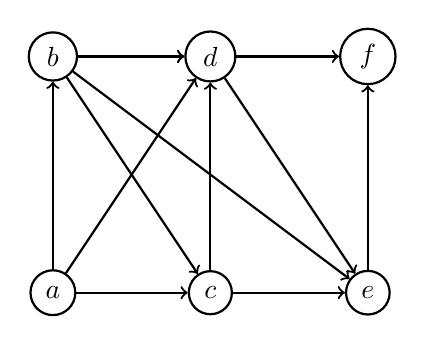
\begin{tikzpicture}
    \begin{scope}[every node/.style={circle,thick,draw}]
      \node (a) at (0,0) {$a$};
      \node (b) at (0,3) {$b$};
      \node (c) at (2,0) {$c$};
      \node (d) at (2,3) {$d$};
      \node (e) at (4,0) {$e$};
      \node (f) at (4,3) {$f$};
    \end{scope}
    \begin{scope}[every edge/.style={draw=black,thick}]
      \path (a) edge[->] (b);
      \path (a) edge[->] (c);
      \path (a) edge[->] (d);
      \path (b) edge[->] (c);
      \path (b) edge[->] (d);
      \path (b) edge[->] (e);
      \path (b) edge[->] (d);
      \path (c) edge[->] (d);
      \path (c) edge[->] (e);
      \path (d) edge[->] (e);         
      \path (e) edge[->] (f);
      \path (d) edge[->] (f);
    \end{scope}
  \end{tikzpicture}
  \end{center}
\begin{solution}
Left for the student.
\end{solution}


\question
The rest of the questions relate to the movie database included with Neo4j.
Kevin Bacon is represented by a node in the database.
Find the \mintinline{cypher}{<id>} of the node.
\begin{solution}
\begin{minted}{cypher}
MATCH
  (n:Actor)
WHERE
  n.name =~ ".*evin.*acon.*"
RETURN
  ID(n);
\end{minted}
\end{solution}


\question
Find a list of the titles of all movies Kevin Bacon has acted in (that are contained in the database).
\begin{solution}
\begin{minted}{cypher}
MATCH
  (a:Actor)-[:ACTS_IN]->(m:Movie)
WHERE
  ID(a) = 759
RETURN
  m.title;
\end{minted}
\end{solution}


\question
Find a list of the titles of all movies Kevin Bacon has acted in, sorted alphabetically.
\begin{solution}
\begin{minted}{cypher}
MATCH
  (a:Actor)-[:ACTS_IN]->(m:Movie)
WHERE
  ID(a) = 759
RETURN
  m.title
ORDER BY
  m.title;
\end{minted}
\end{solution}


\question
Find a list of the titles of all movies Kevin Bacon has acted in, giving only the first five sorted alphabetically.
\begin{solution}
\begin{minted}{cypher}
MATCH
(a:Actor)-[:ACTS_IN]->(m:Movie)
WHERE
  ID(a) = 759
RETURN
  m.title
ORDER BY
  m.title
LIMIT
  5;
\end{minted}
\end{solution}


\question
Find a list of all the names of actors who have acted with Kevin Bacon in a movie, sorted alphabetically.
\begin{solution}
\begin{minted}{cypher}
MATCH
  (kb:Actor {name: "Kevin Bacon"})
    -[:ACTS_IN]->
  (:Movie)<-[:ACTS_IN]-(a:Actor)
WHERE
  a.name <> "Kevin Bacon"
RETURN
  a.name
ORDER BY
  a.name;
\end{minted}
\end{solution}

\question
Find a list of all the names of actors who have acted with an actor who has acted with Kevin Bacon in a movie, sorted alphabetically.
\begin{solution}
  \begin{minted}{cypher}
MATCH
  (kb:Actor {name: "Kevin Bacon"})
    -[:ACTS_IN]->
  (x:Movie)
    <-[:ACTS_IN]-
  (z:Actor)
    -[:ACTS_IN]->
  (y:Movie)
    <-[ACTS_IN]-
  (a:Actor)
RETURN
  DISTINCT a.name
ORDER BY
  a.name;
  \end{minted}
\end{solution}


\question
Find the three nodes representing Kevin Bacon, Elvis Presley and Edward Asner.
\begin{solution}
\begin{minted}{cypher}
MATCH
  (n:Actor), (m:Actor), (o:Actor)
WHERE
  n.name =~ ".*lvis.*sley.*" AND 
  m.name =~ ".*evin.*acon.*" AND 		
  o.name =~ ".*ward.*sner.*"
RETURN
  n, m, o;
\end{minted}
\end{solution}

\question
Find all the titles movies that Kevin Bacon and Edward Asner have acted in together.
\begin{solution}
  \begin{minted}{cypher}
MATCH
  (n:Actor)-[:ACTS_IN]->(i:Movie)<-[:ACTS_IN]-(m:Actor)
WHERE
  ID(n) = 759
  AND ID(m) = 7767
RETURN
  i.title;
  \end{minted}
\end{solution}

\question
Find the titles of all movies that Elvis Presley and Edward Asner have acted in together.
\begin{solution}
  \begin{minted}{cypher}
MATCH
  (n:Actor)-[:ACTS_IN]->(i:Movie)<-[:ACTS_IN]-(m:Actor)
WHERE
  ID(n) = 13543
  AND ID(m) = 7767
RETURN
  i.title;
  \end{minted}
\end{solution}

\question
Find the three nodes representing Kevin Bacon, Elvis Presley and Edward Asner, and all nodes representing any movies that at least two of them have acted in.
\begin{solution}
  \begin{minted}{cypher}
OPTIONAL MATCH
 (n:Actor)-[:ACTS_IN]->(i:Movie)<-[:ACTS_IN]-(m:Actor)
OPTIONAL MATCH
 (n:Actor)-[:ACTS_IN]->(j:Movie)<-[:ACTS_IN]-(o:Actor)
OPTIONAL MATCH
 (m:Actor)-[:ACTS_IN]->(k:Movie)<-[:ACTS_IN]-(o:Actor)
WHERE
  ID(n) = 759
  AND ID(m) = 7767
  AND ID(o) = 13543
RETURN
  n, m, o, i, j, k;
  \end{minted}
\end{solution}

\question
Show that Elvis Presley has a Bacon number of 2.
\begin{solution}
  \begin{minted}{cypher}
MATCH
  p=shortestPath(
    (kb:Actor {name: "Kevin Bacon"})
    -[r:ACTS_IN*]-
    (ep:Actor {name: "Elvis Presley"})
  )
RETURN
  LENGTH(RELATIONSHIPS(p)) / 2 AS BaconNo;
  \end{minted}
\end{solution}

\question
Find the names of all actors with a Bacon number of at most 3.
\begin{solution}
  \begin{minted}{cypher}
MATCH
  (kb:Actor {name: "Kevin Bacon"})
  -[r:ACTS_IN*2..6]-
  (x:Actor)
RETURN
  x.name;
  \end{minted}
\end{solution}

\question
Find the names of all actors with a Bacon number of exactly 3.
\begin{solution}
  \begin{minted}{cypher}
MATCH
  (kb:Actor {name: "Kevin Bacon"})
    -[r:ACTS_IN*6]-
  (x:Actor)
RETURN
  x.name;
  \end{minted}
\end{solution}

\question
\textbf{Extra credit:} Find a distinct list of the types of all the relationships between the \emph{Person} Wes Craven and the \emph{Movie} Scream.
\begin{solution}
  \begin{minted}{cypher}
MATCH
  (n {name: "Wes Craven"})-[r]-(m {title: "Scream"})
RETURN
  TYPE(r)
  \end{minted}
\end{solution}



\end{questions}



\bibliographystyle{plain}
\bibliography{bibliography}
\end{document}
